\documentclass[12pt]{article}
 
\usepackage[margin=1in]{geometry} 
\usepackage{amsmath,amsthm,amssymb}
\usepackage{hyperref}
\usepackage{graphicx}
\usepackage{xcolor}
\usepackage[many]{tcolorbox}
\tcbuselibrary{listings}
\usepackage{listings}

\definecolor{lg}{HTML}{f0f0f0}

\newtcblisting{pycode}{
    colback=lg,
    boxrule=0pt,
    arc=0pt,
    outer arc=0pt,
    top=0pt,
    bottom=0pt,
    colframe=white,
    listing only,
    left=15.5pt,
    enhanced,
    listing options={
        basicstyle=\small\ttfamily,
        keywordstyle=\color{blue},
        language=Python,
        showstringspaces=false,
        tabsize=2,
        numbers=left,
        breaklines=true
    },
    overlay={
        \fill[gray!30]
        ([xshift=-3pt]frame.south west)
        rectangle
        ([xshift=11.5pt]frame.north west);
    }
}

\lstset{
    language=Python,
    basicstyle=\small\ttfamily,
}

 
\begin{document}
 
\title{Home Assignment 1}
\author{Cristian Manuel Abrante Dorta - 888248\\
CS-E4650 - Methods of data mining}

\maketitle
\section{Task 1}
\label{sec:task-1}

\subsection{Perform K-means and evaluate the goodness of clustering using
Silhouette Coefficient, Calinski Harabasz and Davies-Bouldin indices.
K = 2.}

An analysis of the results of the K-Means algorithm have been performed for three different values of K, and three indexes respectively. In order to reproduce the results, the random seed of the generator have been set to the value of $10$, obtaining the following results:

\begin{table}[h]
\centering
\begin{tabular}{c|ccc}
       & Avg. Silhouette coefficient & Calinski-Harabsz index & Davies-Bouldin score \\ \hline
$K = 2$  & 0.5587                 & 847.702                & 0.6216               \\
$K = 5$  & 0.4006                 & 778.4351               & 0.9299               \\
$K = 10$ & 0.3489                 & 593.5482               & 1.0729              \\

\end{tabular}
\caption{Results of different indexes for K = 2, K= 5 and K=10}
\end{table}

Also, those results could be seen graphically

\subsection{What is the optimal $K$ and why?}

For answering this question, it is needed an analysis of the performance of the K-means algorithm for each index, and each value of $k$.

\subsubsection{Silhouette coefficient}

The silhouette score indicates how each data point is close to the cluster it was matched by the algorithm, and how far it is from the other clusters (the neighbour clusters). This score vary from $[-1, +1]$, and can be calculated for each data point, as it is represented in Figure :

\begin{figure}[H]
   \begin{minipage}{0.32\textwidth}
     \centering
     \includegraphics[width=\linewidth]{pl}
     \caption{First execution}
     \label{fig:task-2-v1}
   \end{minipage}\hfill
   \begin{minipage}{0.32\textwidth}
     \centering
     \includegraphics[width=\linewidth]{exercise-1/report/img/task-2-v2.png}
     \caption{Second execution}
     \label{fig:task-2-v2}
   \end{minipage}
   \begin{minipage}{0.32\textwidth}
     \centering
     \includegraphics[width=\linewidth]{exercise-1/report/img/task-2-v3.png}
     \caption{Third execution}
     \label{fig:task-2-v3}
   \end{minipage}
\end{figure}



































\section{Task 2}
To embed code snippets in the report, you can use the \texttt{pycode} environment.

\begin{pycode}
def main():
    print("Hello World")
\end{pycode}

\section{Question 1}

If you add a figure, you can refer to it using Figure.~\ref*{fig:fig1}.

\begin{figure}[h] 
	\centering  % Remember to centre the figure
    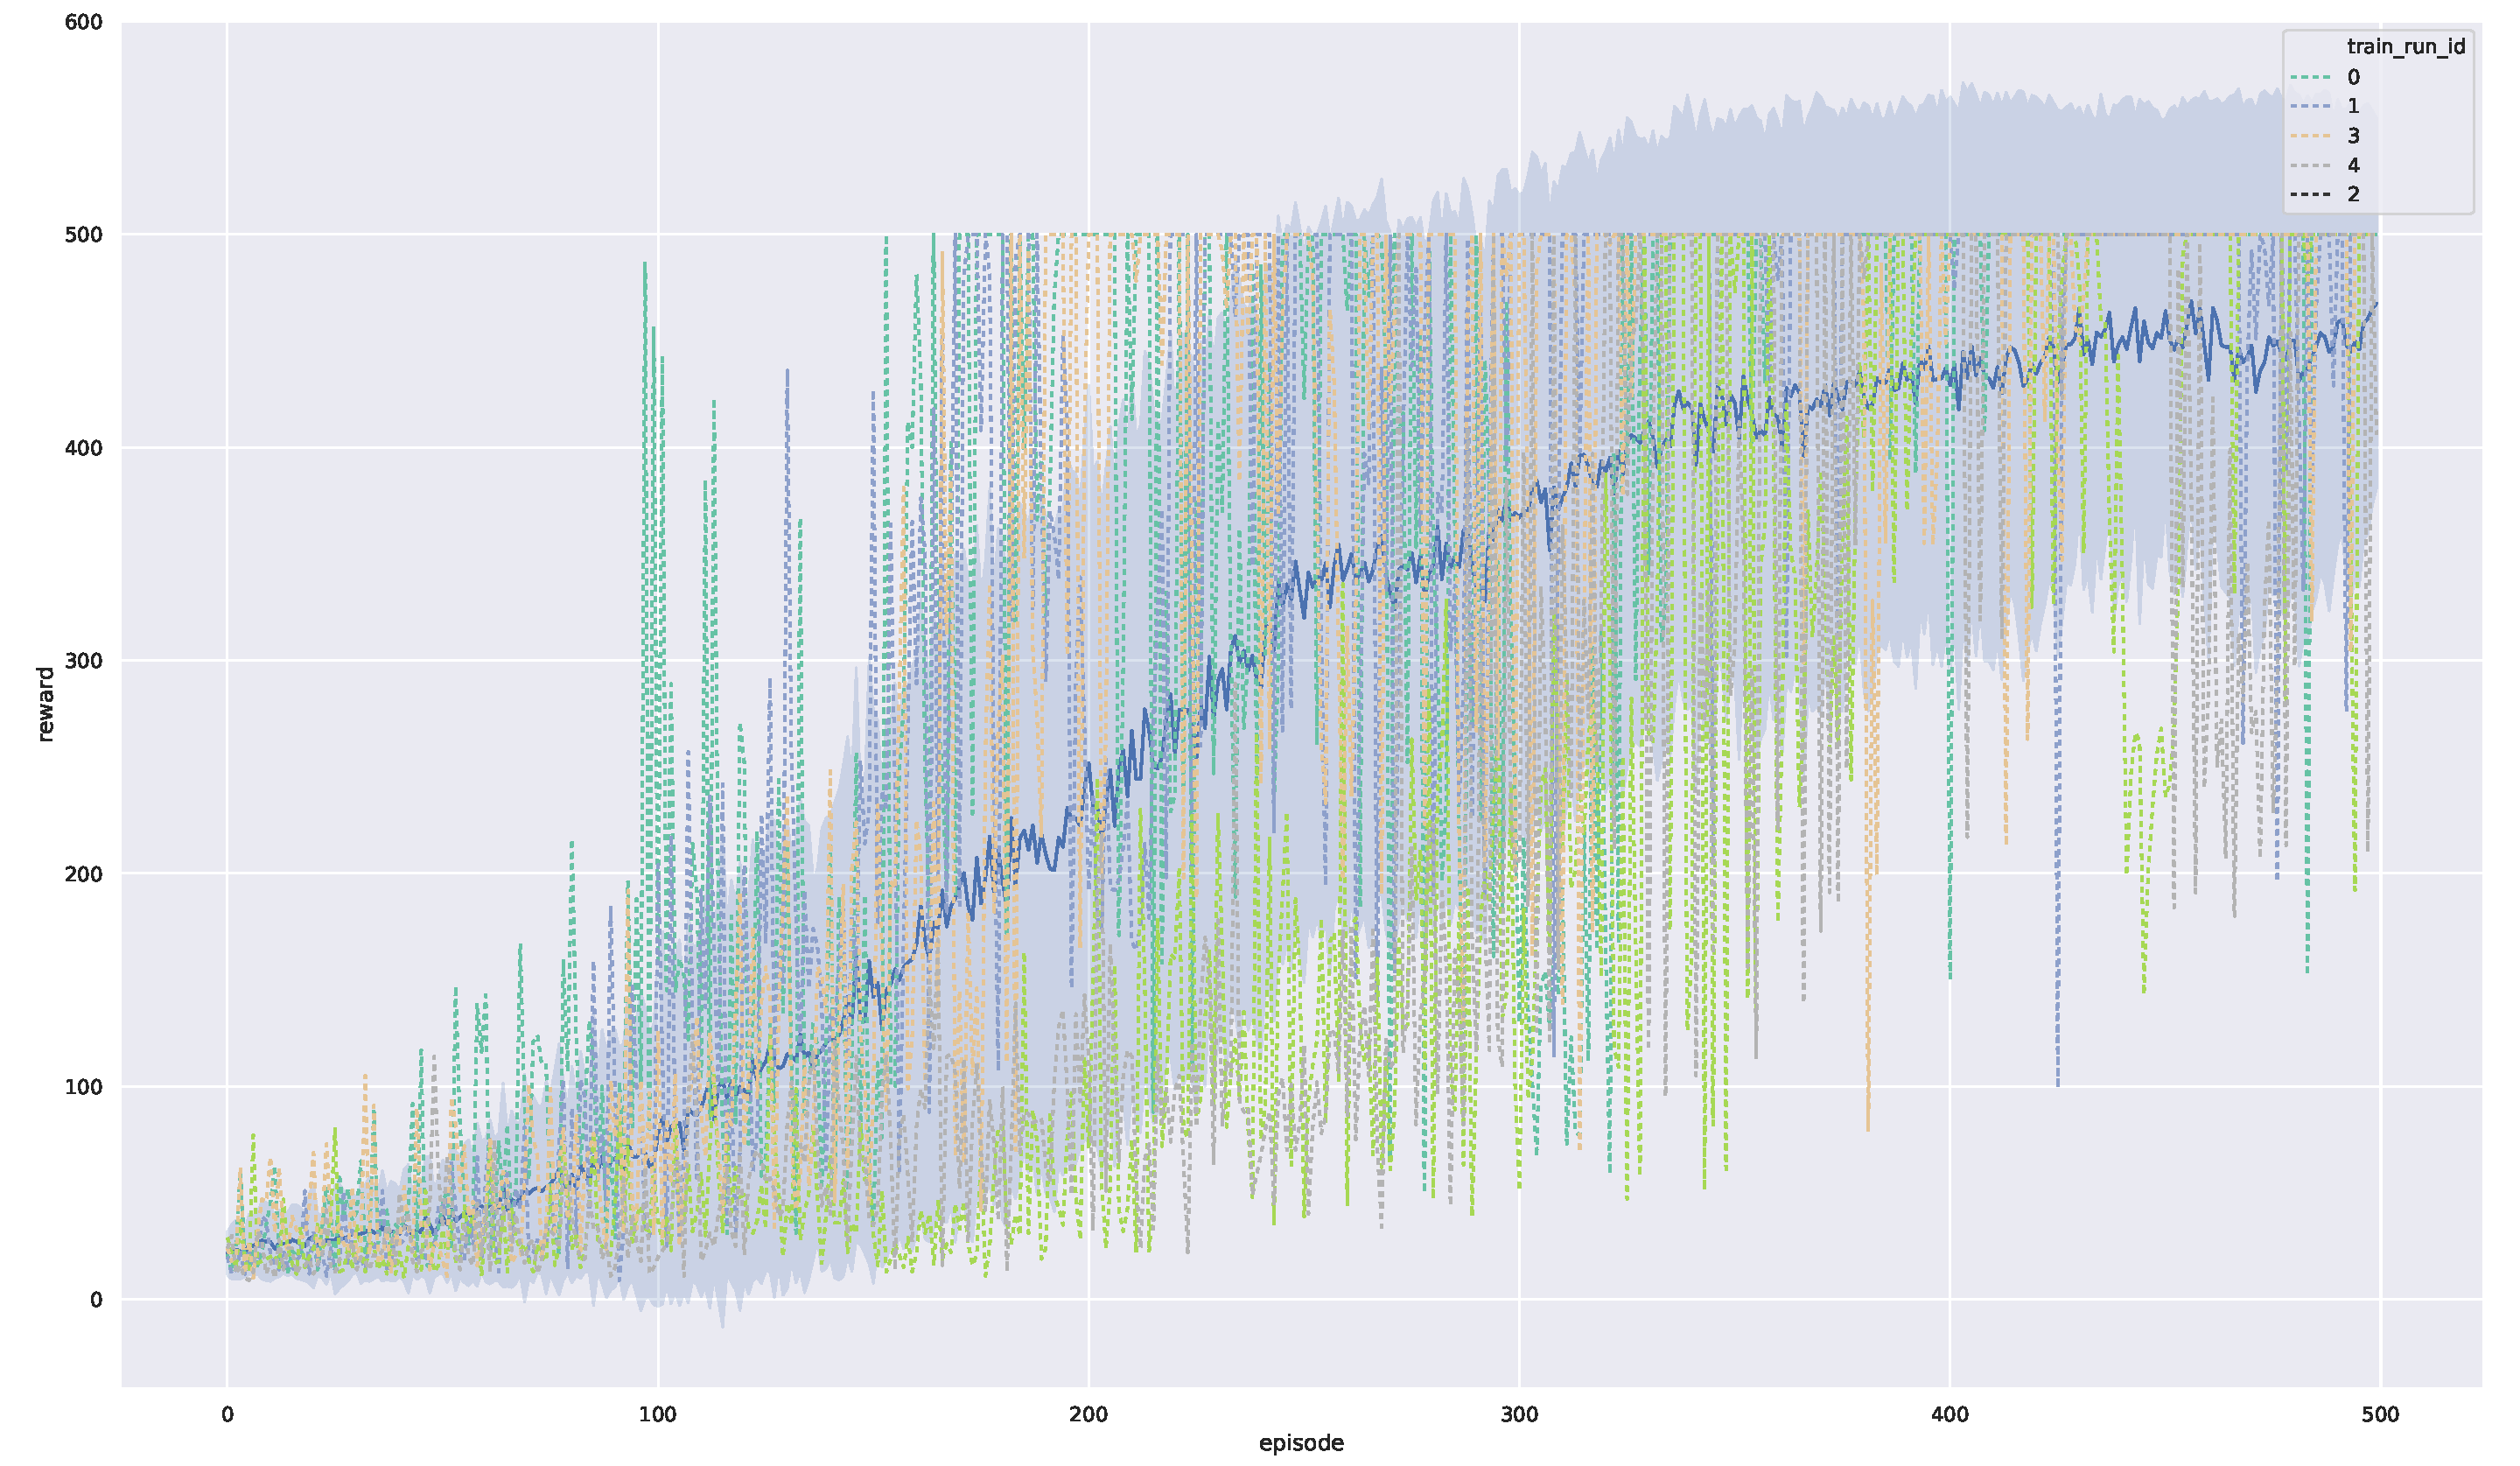
\includegraphics[width=0.3\columnwidth]{img/training.pdf}
	\caption{This is a sample figure.}
	\label{fig:fig1}
\end{figure}

\bibliographystyle{ieeetr}
\bibliography{bibliography}  % Modify template with your bibliography name
\end{document}
